\documentclass[12pt,letterpaper,twocolumn,openany,nodeprecatedcode,bg=none]{dndbook}
\usepackage[english]{babel}
\usepackage[utf8]{inputenc}
\usepackage{longtable,booktabs,array}
\usepackage{calc}
\usepackage{etoolbox}
\usepackage{caption}
\AtBeginEnvironment{longtable}{\small}

% Fix for Pandoc 3.1.7+ image handling
\providecommand{\pandocbounded}[1]{#1}

% Pandoc's compact list helper
\providecommand{\tightlist}{%
  \setlength{\itemsep}{0pt}\setlength{\parskip}{0pt}}

% Remove "Figure N:" prefix from captions
\captionsetup{labelformat=empty}

% Remove section numbering
\setcounter{secnumdepth}{0}

\begin{document}

\title{Fighter}
\author{Class Handbook}
\date{}
\maketitle

\onecolumn

\emph{Your trusty class handbook for the Old Scrolls roleplaying game.}

\clearpage

\begin{figure}
\centering
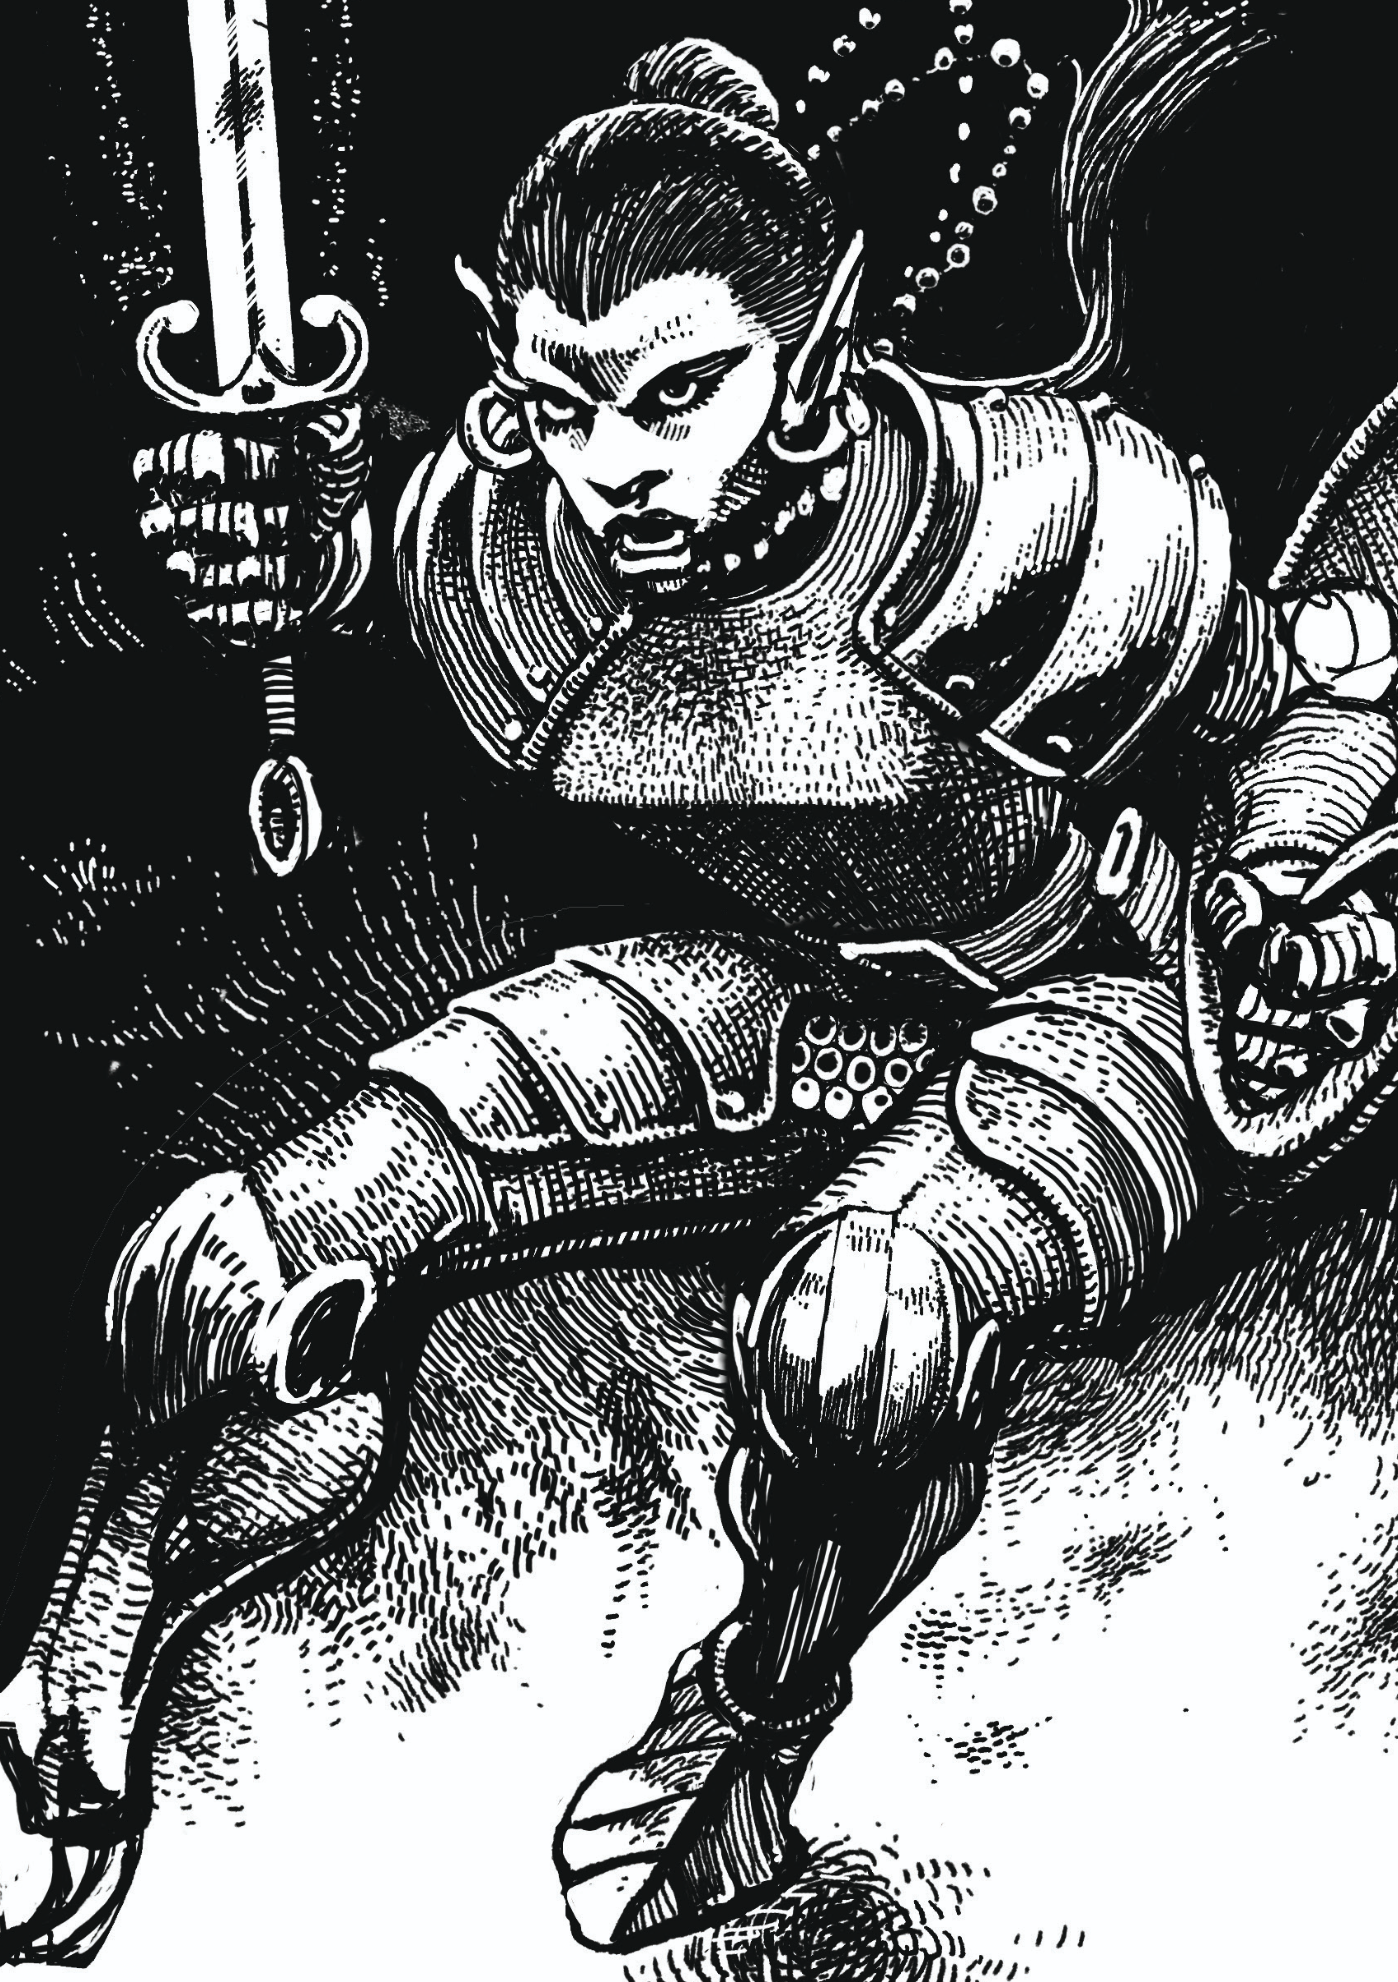
\includegraphics[width=1\linewidth,height=\textheight,keepaspectratio]{orcFighter.png}
\caption{\emph{Never underestimate a fighter with their sword}}
\end{figure}

\clearpage

\section{Fighter}\label{fighter}

The classic. This is somebody with some weapon's training, some
equipment, and a burning desire to start adventuring with some friends.
Their specific training can be as vague or specific as you like. A
perfect blank slate to start building a character from.

\subsection{Core Fighter Traits}\label{core-fighter-traits}

\begin{longtable}[]{@{}
  >{\raggedright\arraybackslash}p{(\linewidth - 2\tabcolsep) * \real{0.2542}}
  >{\raggedright\arraybackslash}p{(\linewidth - 2\tabcolsep) * \real{0.7458}}@{}}
\toprule\noalign{}
\begin{minipage}[b]{\linewidth}\raggedright
\textbf{Primary Ability}
\end{minipage} & \begin{minipage}[b]{\linewidth}\raggedright
Strength
\end{minipage} \\
\midrule\noalign{}
\endhead
\bottomrule\noalign{}
\endlastfoot
\textbf{Hit Points} & 14 at 1st level, 10 per level gained after 1st \\
\textbf{Saving Throw Proficiencies} & Strength, Constitution \\
\textbf{Skill Proficiencies} & Choose any 2 skills. If you choose a
skill you already have, you gain expertise with it. \\
\textbf{Weapon Proficiencies} & Choose 4: Blade, Blunt, Bow, Mechanical,
Polearm, and Shield \\
\textbf{Starting Equipment} & Breastplate or Scale Mail or Chain Mail,
Open Helm, Greatsword, Sabre, Large Shield. \\
\end{longtable}

\subsection{Fighter Features}\label{fighter-features}

\begin{longtable}[]{@{}
  >{\raggedright\arraybackslash}p{(\linewidth - 4\tabcolsep) * \real{0.0714}}
  >{\raggedright\arraybackslash}p{(\linewidth - 4\tabcolsep) * \real{0.1571}}
  >{\raggedright\arraybackslash}p{(\linewidth - 4\tabcolsep) * \real{0.7714}}@{}}
\toprule\noalign{}
\begin{minipage}[b]{\linewidth}\raggedright
Level
\end{minipage} & \begin{minipage}[b]{\linewidth}\raggedright
Proficiency
\end{minipage} & \begin{minipage}[b]{\linewidth}\raggedright
Class Features
\end{minipage} \\
\midrule\noalign{}
\endhead
\bottomrule\noalign{}
\endlastfoot
1 & +2 & Fighting Style, Gritty Recovery, Weapon Specialization \\
2 & +2 & Action Surge \\
3 & +2 & Combat Mastery, Fighter's Talent \\
4 & +2 & Ability Score Improvement \\
5 & +3 & Mighty Warrior \\
6 & +3 & Ability Score Improvement \\
7 & +3 & Tactical Reflexes \\
8 & +3 & Ability Score Improvement, Combat Supremacy \\
9 & +4 & Indomitable \\
10 & +4 & Mighty Surge \\
\end{longtable}

\twocolumn

\subsection{Fighter Features}\label{fighter-features-1}

As a fighter, you gain the following class features when you reach the
specified levels. These features are listed on the Fighter Features
table.

\subsection{Level 1: Fighting Style}\label{level-1-fighting-style}

You are trained in one specific style of fighting.

\begin{itemize}
\tightlist
\item
  \textbf{Bulwark.} Once per turn when a hostile creature in melee range
  attempts to move, it must make a Dexterity saving throw (DC 8 + your
  proficiency bonus + your Strength modifier). If it fails, it cannot
  move that turn.
\item
  \textbf{Berserker.} Once per turn when you drop a target to 0 hit
  points with an attack, you may make one additional attack.
\item
  \textbf{Duelist.} You gain +2 AC while wearing armor that weighs 20
  pounds or less and are not using a shield.
\item
  \textbf{Guardian.} You gain +1 AC. If a hostile creature in melee
  range attacks, you may choose its target. You must choose a creature
  hostile to it, such as yourself.
\item
  \textbf{Monster Slayer.} You gain a +2 bonus to damage rolls against
  creatures that are larger than you.
\item
  \textbf{Sharpshooter.} You add double your proficiency bonus to attack
  rolls with ranged attacks.
\item
  \textbf{Stalwart.} You gain a bonus to your maximum hit points equal
  to your level. While you are at half hit points or less, you regain
  hit points at the start of your turn equal to your Constitution
  modifier.
\item
  \textbf{Warrior Mage.} You gain a wizard cantrip of your choice and
  can cast one wizard spell. Each time you gain a level, you can swap
  those choices for different options. You use the rules for casting
  spells as per the wizard class.
\item
  \textbf{Warrior Mystic.} You gain a mystic cantrip of your choice and
  can cast one mystic spell. Each time you gain a level, you can swap
  those choices for different options. You use the rules for casting
  spells as per the mystic class.
\end{itemize}

\subsection{Level 1: Gritty Recovery}\label{level-1-gritty-recovery}

You have an incredible reservoir of durability that carries you through
even the most difficult battles. At the start of your turn, you can
regain hit points equal to half your maximum hit points.

Once you use this feature, you cannot use it again until you finish a
long rest.

\subsection{Level 1: Weapon
Specialization}\label{level-1-weapon-specialization}

Pick a weapon you are proficient with. You add your proficiency bonus to
damage rolls with it. After an extended period of downtime, you can swap
this choice to a different weapon.

\subsection{Level 2: Action Surge}\label{level-2-action-surge}

You can push yourself beyond your normal limits for a moment. On your
turn, you can take one additional action. Once you use this feature, you
can't do so again until you finish a short or long rest.

\subsection{Level 3: Combat Mastery}\label{level-3-combat-mastery}

You have a combat mastery die, a d10. You regain expended dice at the
start of your turn. You can use a die in the following ways:

\begin{itemize}
\tightlist
\item
  If you miss with an attack, roll the die and add the result to your
  attack roll. This bonus can turn a miss into a hit.
\item
  If you hit with an attack, roll the die and add the result as a bonus
  to your damage roll.
\item
  If you are hit by an attack, roll the die and add the result to your
  AC. This bonus can potentially turn a hit into a miss.
\end{itemize}

\textbf{Action Surge.} When you use Action Surge, you regain all
expended combat mastery dice.

\subsection{Level 3: Fighter's Talent}\label{level-3-fighters-talent}

Pick a skill that you are proficient with or have expertise with. When
you make a check using that skill, you can expend a combat mastery die
to augment your check. Roll your combat mastery die and add the result
as a bonus to that check. You can use up to one such die per check.

\subsection{Level 4: Ability Score
Improvement}\label{level-4-ability-score-improvement}

You gain a +1 bonus to two abilities of your choice.

\subsection{Level 5: Mighty Warrior}\label{level-5-mighty-warrior}

As an attack action, you can make two weapon attacks.

\subsection{Level 6: Ability Score
Improvement}\label{level-6-ability-score-improvement}

You gain a +1 bonus to two abilities of your choice.

\subsection{Level 7: Tactical Reflexes}\label{level-7-tactical-reflexes}

You add your proficiency bonus to initiative rolls. The first time you
take a turn after rolling initiative, you may move one additional time.

\subsection{Level 8: Ability Score
Improvement}\label{level-8-ability-score-improvement}

You gain a +1 bonus to two abilities of your choice.

\subsection{Level 8: Combat Supremacy}\label{level-8-combat-supremacy}

You now have two combat mastery dice. Both are d10s. You can apply one
or both to a given roll.

\subsection{Level 9: Indomitable}\label{level-9-indomitable}

When you roll a saving throw or a death save, you can add your level as
a bonus to it. You can't use this feature again until you finish a long
rest. You can choose to use this benefit after learning if you succeed
or fail, potentially turning failure to success.

\subsection{Level 10: Mighty Surge}\label{level-10-mighty-surge}

When you use your Action Surge, you gain advantage on all tests you make
until your next turn.

\onecolumn

\begin{figure}
\centering
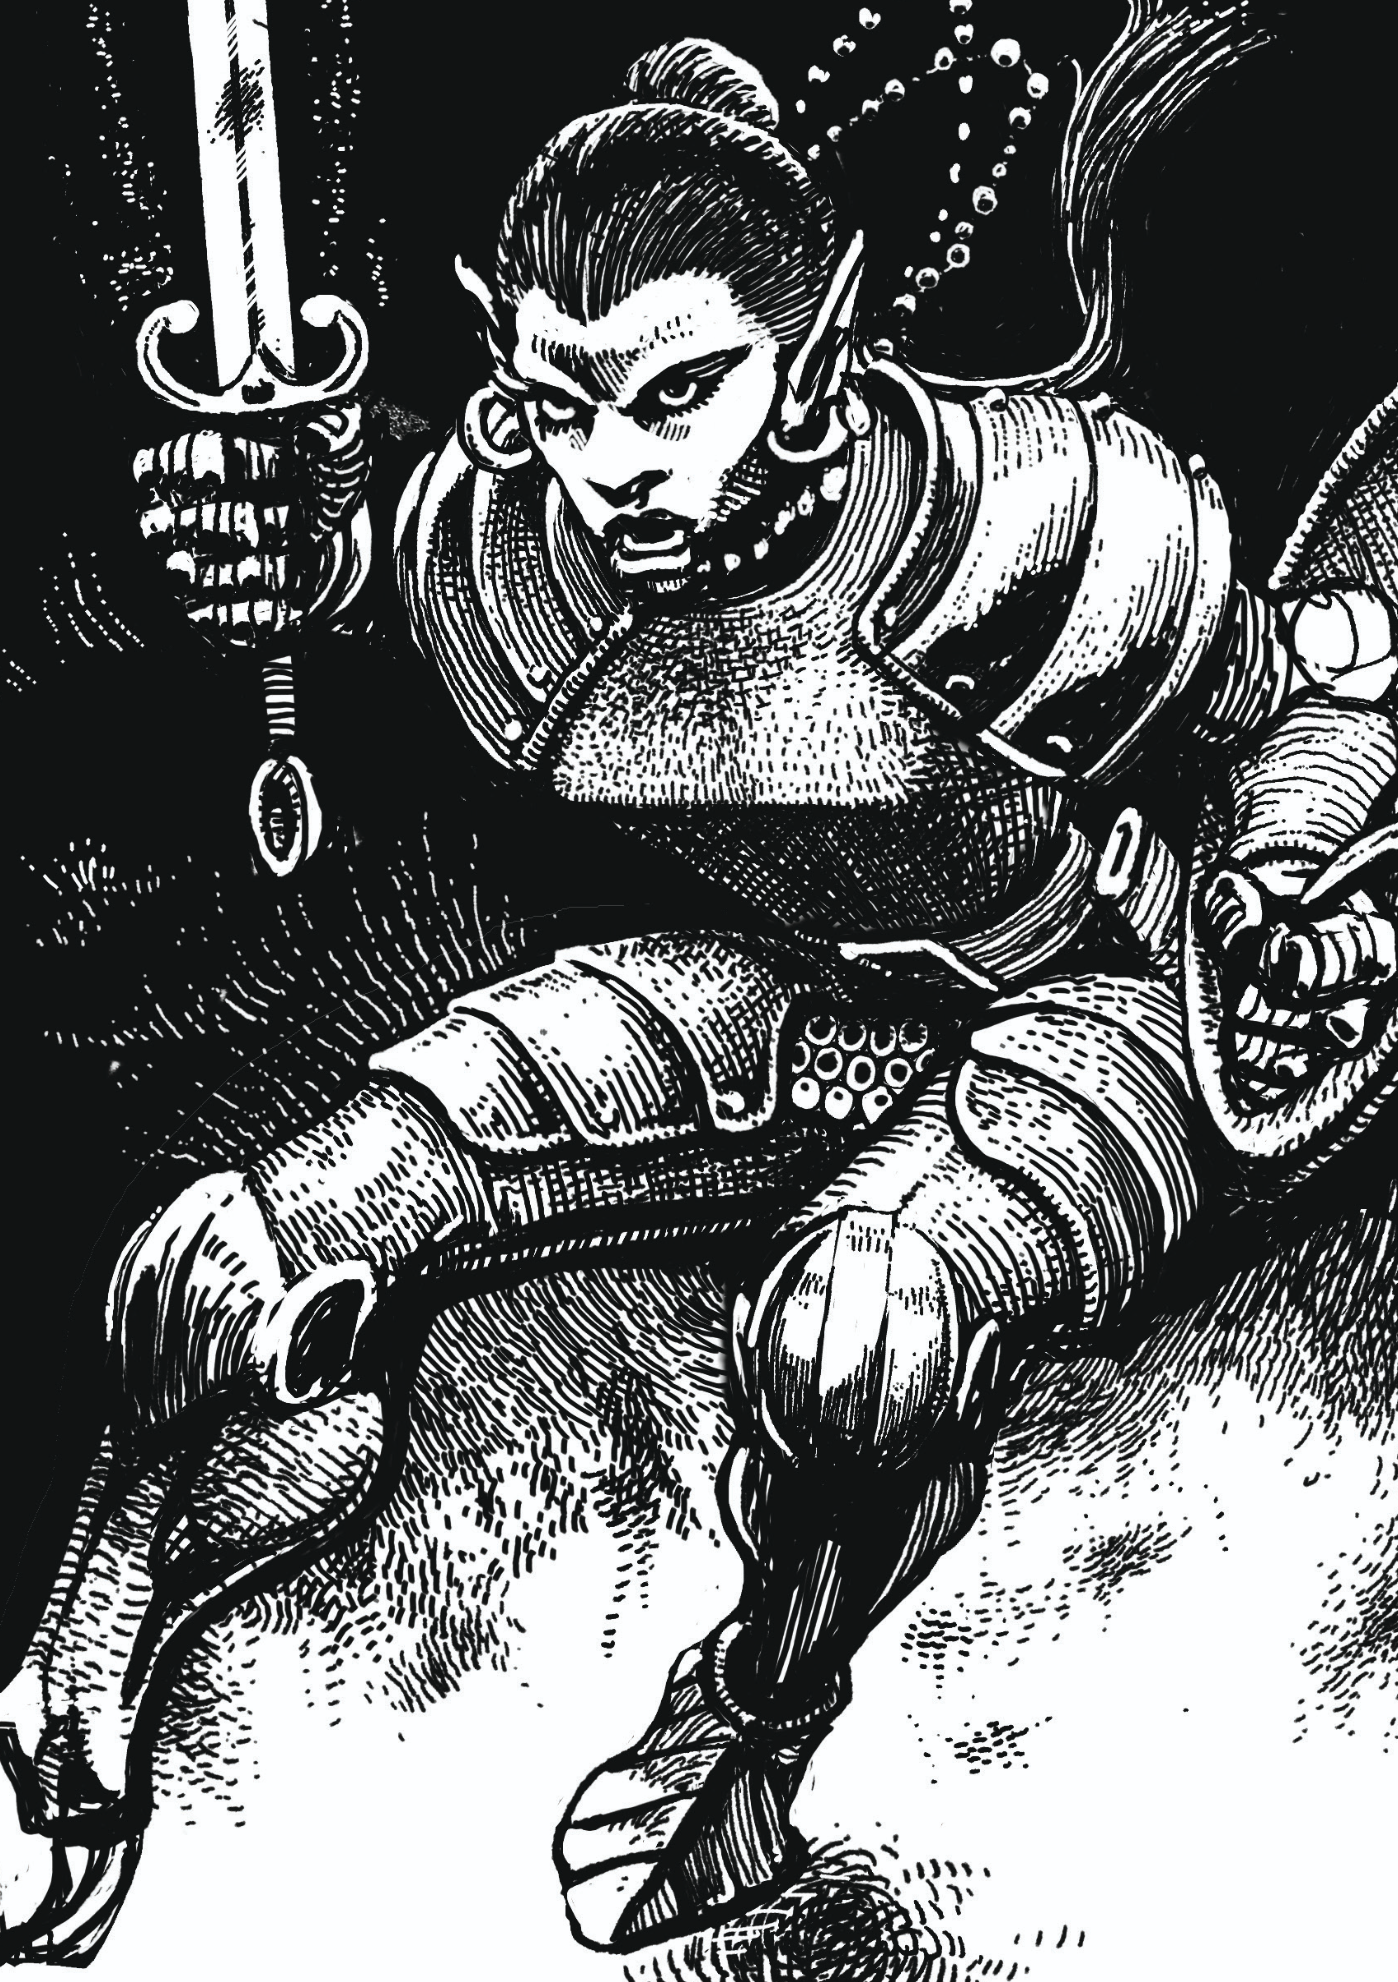
\includegraphics[width=1\linewidth,height=\textheight,keepaspectratio]{orcFighter.png}
\caption{\emph{Never underestimate a fighter with their sword}}
\end{figure}

\clearpage

\emph{The fighter class handbook.}

\end{document}